\documentclass{article}
%%%%%%%%%%%%%
% Loads packages
%%%%%%%%%%%%%
\usepackage[table]{xcolor}
\usepackage[utf8]{inputenc}
\usepackage[colorlinks=true,linkcolor=blue]{hyperref}
\usepackage{geometry} %package needed to set margins
\usepackage{fancyhdr}
\usepackage{graphicx}
\usepackage{amsmath}
\usepackage{amsthm}
\usepackage{mdframed}
\usepackage{tikz}
\usetikzlibrary{arrows.meta}
\usetikzlibrary{decorations.markings}
\usepackage{amsfonts}
\usepackage{wasysym}

\usepackage{listings}% http://ctan.org/pkg/listings
\lstset{
  basicstyle=\ttfamily,
  mathescape
}


\pagestyle{fancy}
\fancyhf{}
\chead{\textbf{Homework 9}}
\lhead{Math 213, Fall 2024}
\rhead{Due Sunday, 11/10 at 11:59pm}

%%%%%%%%%%%%%
% Sets margins
%%%%%%%%%%%%%
\newgeometry{left=1.5in,right=1in,top=1in,bottom=1in}
\setlength\headsep{3pt}

%%%%%%%%%%%%%
% Creates problem and solution environments
%%%%%%%%%%%%%

% Solution Environment
\newenvironment{solution}{\begin{proof}[Solution]}{\end{proof}}

% Problem Environment
\newenvironment{problem}[1]
    {\begin{mdframed}[default]
    \textbf{Problem #1:}
    }
    {\end{mdframed}
    }
    
%%%%%%%%%%%
% Custom Commands
%%%%%%%%%%%
\newcommand{\gOne}{\cellcolor{green!50!white} 1}
\newcommand{\rZero}{\cellcolor{red!50!white} 0}

\begin{document}

\begin{problem}{\S 9.5 - 3(c,d,e)}
Which of these relations on the set of all functions from $\mathbb{Z}$ to $\mathbb{Z}$ are equivalence relations? Determine the properties of an equivalence relation that the others lack.
\begin{itemize}
    \item[(c)] $\{ (f,g)~:~ f(x)-g(x) = 1 \textrm{ for all } x \in \mathbb{Z}\}$.
    \item[(d)] $\{ (f,g)~: \textrm{ for some } C \in \mathbb{Z}, \textrm{ for all } x \in \mathbb{Z}, f(x) - g(x) = C \}$.
    \item[(e)] $\{ (f,g)~|~f(0) = g(1) \textrm{ and } f(1) = g(0) \}$.
\end{itemize}
\end{problem}

\begin{problem}{\S 9.5 - 22}
Determine whether the relation with the directed graph shown is an equivalence relation.
\begin{center}
    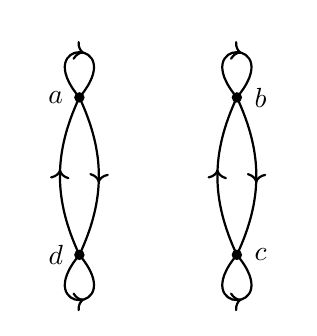
\begin{tikzpicture}
    \begin{scope}[thick,decoration={
            markings,
            mark=at position 0.54 with {\arrow{>}}}
            ] 
            
        % draws vertices
        \node[circle, fill=black,scale = 0.4] at (0,0){};
        \node[circle, fill=black,scale = 0.4] at (0,2){};
        \node[circle, fill=black,scale = 0.4] at (2,2){};
        \node[circle, fill=black,scale = 0.4] at (2,0){};
        
        % draws directed edges
        \draw[postaction={decorate},out=115,in=-115] (0,0) to (0,2);
        \draw[postaction={decorate},out=-65,in=65] (0,2) to (0,0);
        \draw[postaction={decorate},out=115,in=-115] (2,0) to (2,2);
        \draw[postaction={decorate},out=-65,in=65] (2,2) to (2,0);
        \draw[scale=2,postaction={decorate}] (0,0) to[out=-130,in=-50,loop] (0,0);
        \draw[scale=2,postaction={decorate}] (1,0) to[out=-130,in=-50,loop] (1,0);
        \draw[scale=2,postaction={decorate}] (1,1) to[out=130,in=50,loop] (1,1);
        \draw[scale=2,postaction={decorate}] (0,1) to[out=130,in=50,loop] (0,1);
        
        % labels vertices
        \node at (-0.3,0) {$d$};
        \node at (-0.3,2) {$a$};
        \node at (2.3,2) {$b$};
        \node at (2.3,0) {$c$};
    \end{scope}
    \end{tikzpicture}
\end{center}
\end{problem}

\begin{problem}{\S 9.5 - 24(a,b)}
Determine whether the relations represented by these binary matrices are equivalence relations.
\begin{itemize}
    \item[(a)] $\begin{bmatrix} 1 & 1 & 1 \\ 0 & 1 & 1 \\ 1 & 1 & 1 \end{bmatrix}$
    \item[(b)] $\begin{bmatrix} 1 & 0 & 1 & 0 \\ 0 & 1 & 0 & 1 \\ 1 & 0 & 1 & 0 \\ 0 & 1 & 0 & 1 \end{bmatrix}$
\end{itemize}
\end{problem}

\begin{problem}{\S 9.5 - 30(a,b)}
What are the equivalence classes of these bit strings for the equivalence relation
\[ R = \{ (x,y)~:~ x \textrm{ and } y \textrm{ are binary strings of length three or more that agree in the first three bits}\} \]
\begin{itemize}
    \item[(a)] 010
    \item[(b)] 1011
\end{itemize}
\end{problem}

\begin{problem}{\S 9.5 - 44(a,b,e)}
Which of these collections of subsets are partitions of the set of integers?
\begin{itemize}
    \item[(a)] the set of even integers and the set of odd integers.
    \item[(b)] the set of positive integers and the set of negative integers.
    \item[(e)] the set of integers not divisible by 3, the set of even integers, and the set of integers that leave a remainder of 3 when divided by 6.
\end{itemize}
\end{problem}

\begin{problem}{\S 9.5 - 48(a)}
List the ordered pairs in the equivalence relation produced by the following partition of $\{ a, b, c, d, e, f, g \}$:
\[ \{ a, b \}, \{ c, d \}, \{ e, f, g \} \]
\end{problem}

\begin{problem}{\S 10.1 - 28}
Describe a graph model that represents a subway system in a large city. Should edges be directed or undirected? Should multiple edges be allowed? Should loops be allowed?
\end{problem}

\begin{problem}{\S 10.2 - 8}
Determine the number of vertices and edges and find the in-degree and out-degree of each vertex for the following graph:
\begin{center}
    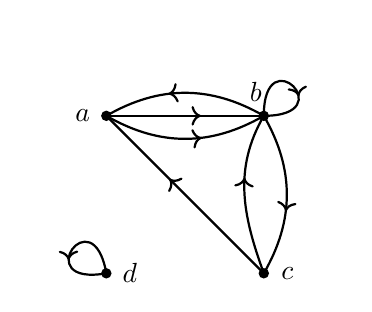
\begin{tikzpicture}
    \begin{scope}[thick,decoration={
            markings,
            mark=at position 0.6 with {\arrow{>}}}
            ]
            
            % draws vertices
            \node[circle, fill=black,scale = 0.4] at (0,0){};
            \node[circle, fill=black,scale = 0.4] at (2,0){};
            \node[circle, fill=black,scale = 0.4] at (0,2){};
            \node[circle, fill=black,scale = 0.4] at (2,2){};
            
            % labels vertices
            \node at (-0.3,2) {$a$};
            \node at (1.9,2.3) {$b$};
            \node at (2.3,0) {$c$};
            \node at (0.3,0) {$d$};
            
            % draws edges
            \draw[postaction={decorate}] (2,0) to (0,2);
            \draw[postaction={decorate}] (0,2) to (2,2);
            \draw[postaction={decorate},out=-30,in=210] (0,2) to (2,2);
            \draw[postaction={decorate},out=150,in=30] (2,2) to (0,2);
            \draw[postaction={decorate},out=-60,in=60] (2,2) to (2,0);
            \draw[postaction={decorate},out=110,in=240] (2,0) to (2,2);
            
            % draws loops
            \draw[scale=2,postaction={decorate}] (0,0) to[out=100, in=190,loop] (0,0);
            \draw[scale=2,postaction={decorate}] (1,1) to[out=90, in=0,loop] (1,1);
    \end{scope}
    \end{tikzpicture}
\end{center}
\end{problem}

\begin{problem}{\S 10.2 - 10}
For the graph in Problem $\S 10.2 - 8$, determine the sum of the in-degrees of the vertices and the sum of the out-degree of the vertices directly. Show that they are both equal to the number of edges in the graph.
\end{problem}

\begin{problem}{\S 10.2 - 35(a,b,c)}
How many vertices and how many edges do these graphs have?
\begin{itemize}
    \item[(a)] $K_n$.
    \item[(b)] $C_n$.
    \item[(c)] $W_n$.
\end{itemize}
\end{problem}

\begin{problem}{\S 10.2 - 37(a,b,c)}
Find the degree sequence of each of the following graphs.
\begin{itemize}
    \item[(a)] $K_4$.
    \item[(b)] $C_4$.
    \item[(c)] $W_4$.
\end{itemize}
\end{problem}


\end{document}